\chapter*{Cochabamba et le parc de Torotoro\markboth{Cochabamba et le parc de Torotoro}{}}
\section*{28 avril 2015}
Départ de Sucre direction Cochabamba. Beaucoup de descente le premier jour, les températures deviennent plus élevées. 

 

\begin{center} 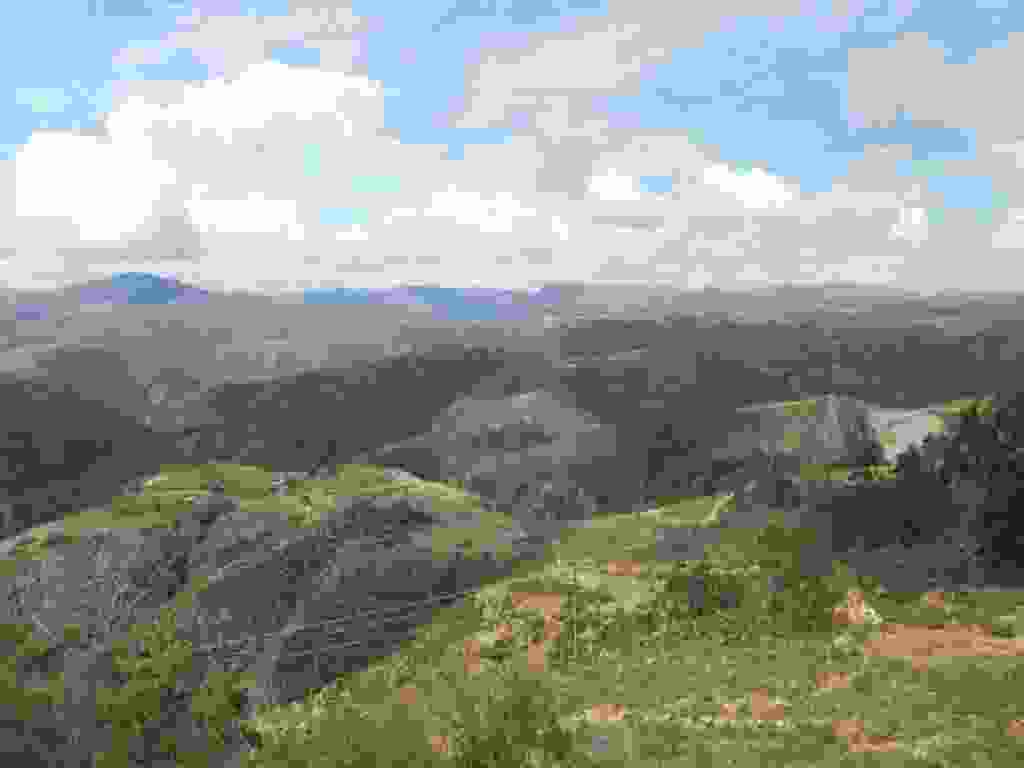
\includegraphics[width=\mywidth]{../wp-content/uploads/2015/04/wpid-wp-1429714724768-1024x768.jpg} \end{center}

 

 

\begin{center} 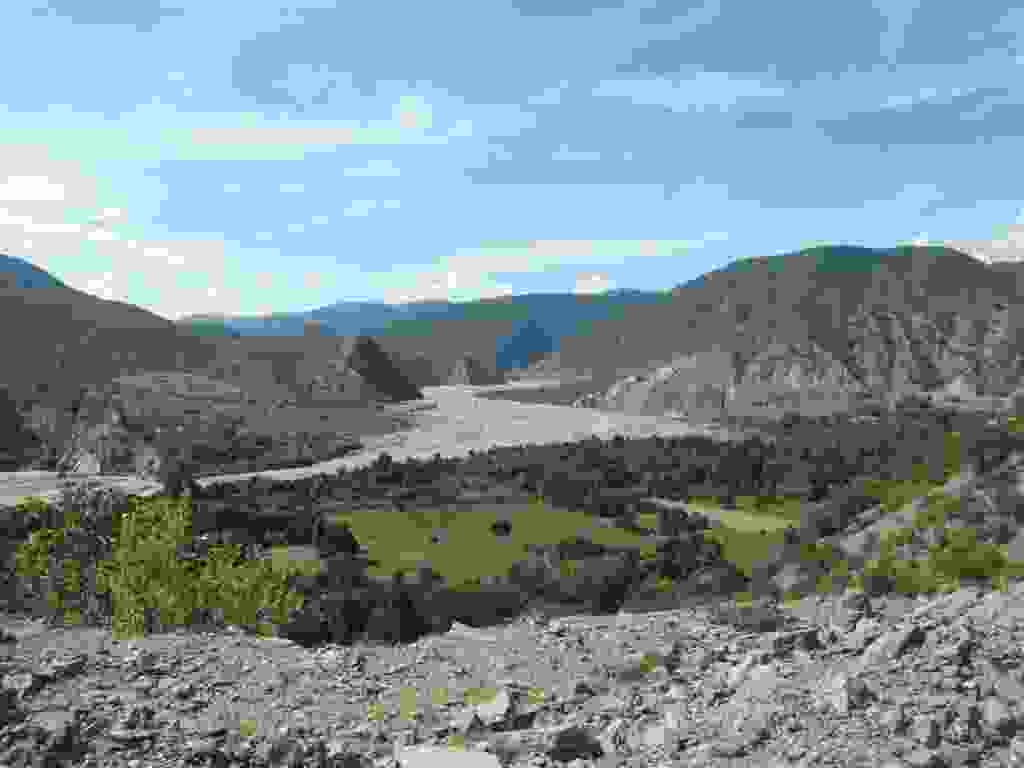
\includegraphics[width=\mywidth]{../wp-content/uploads/2015/04/wpid-wp-1429714753090-1024x768.jpg} \end{center}

 

 

\begin{center} 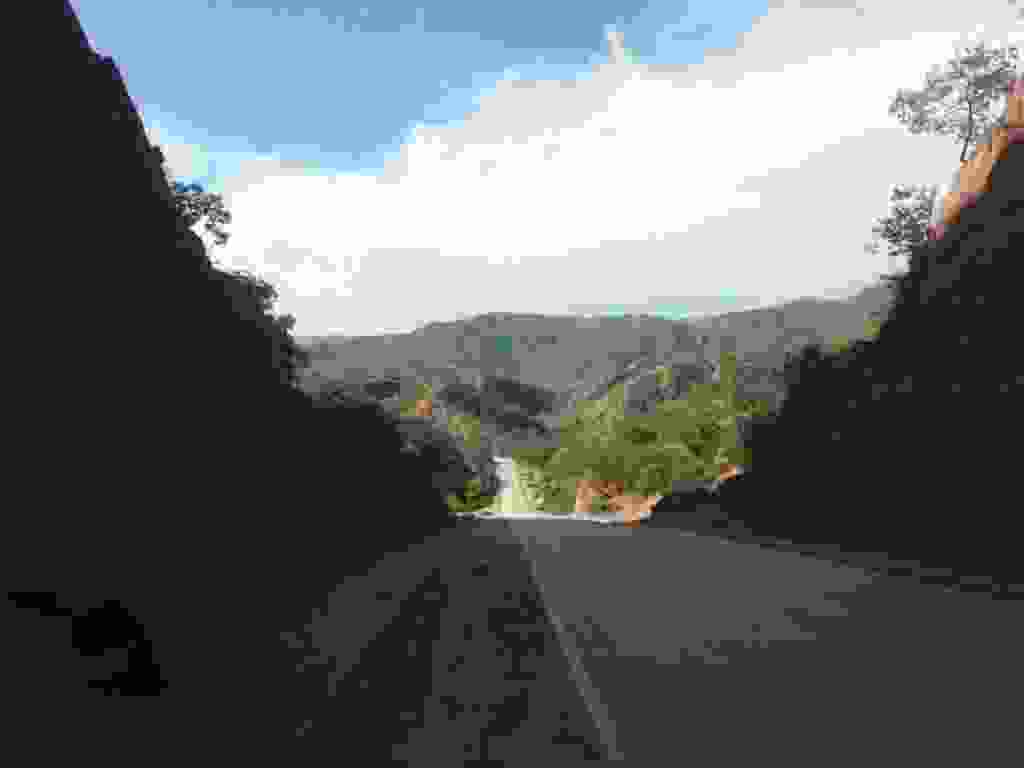
\includegraphics[width=\mywidth]{../wp-content/uploads/2015/04/wpid-wp-1429714770711-1024x768.jpg} \end{center}

 

 Premier bivouac où il a fait très chaud et avec la compagnie des moustiques. 

 

\begin{center} 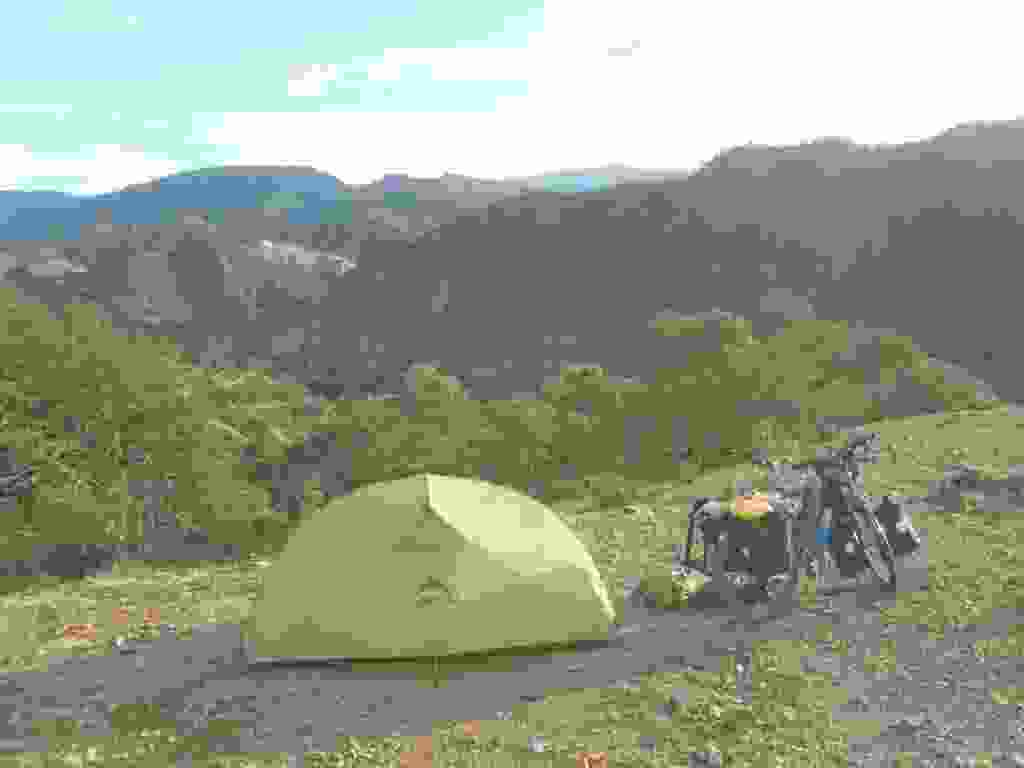
\includegraphics[width=\mywidth]{../wp-content/uploads/2015/04/wpid-wp-1429714848743-1024x768.jpg} \end{center}

 

 En traversant un village le lendemain, je suis arrêté par un homme qui me dit qu'il est le chef du village. 

 

\begin{center} 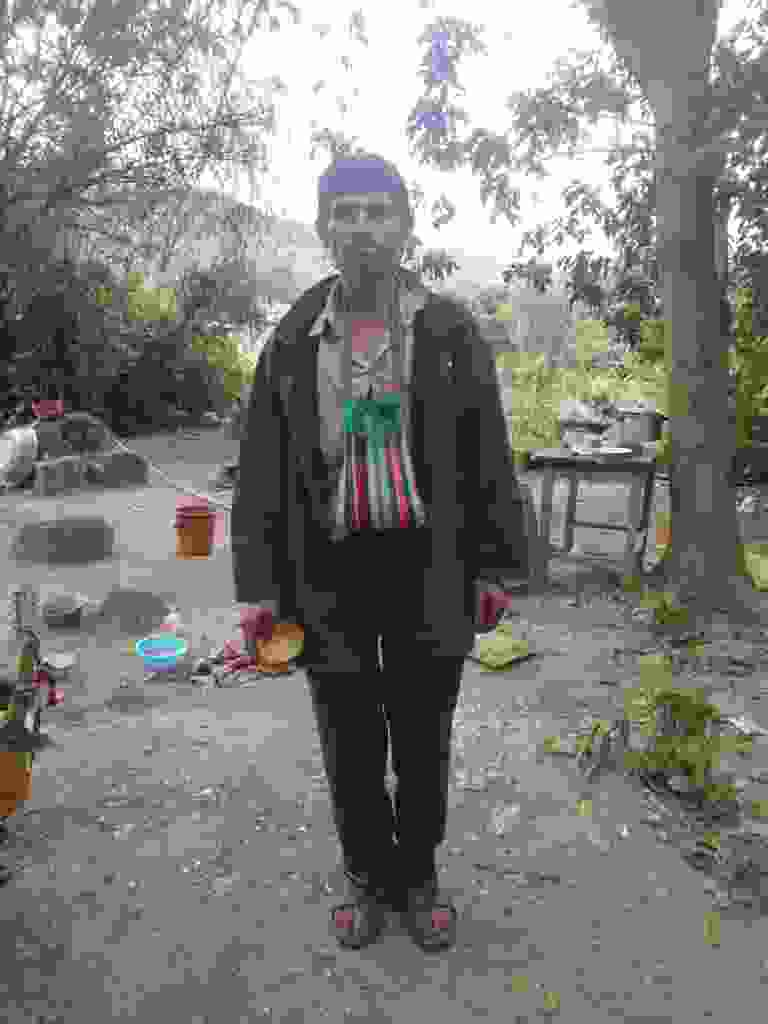
\includegraphics[width=\mywidth]{../wp-content/uploads/2015/04/wpid-wp-1429715140310-768x1024.jpg} \end{center}

 

 Il m'invite à boire un coup avec ses amis, manifestement ils n'en sont pas au premier verre. 

 

\begin{center} 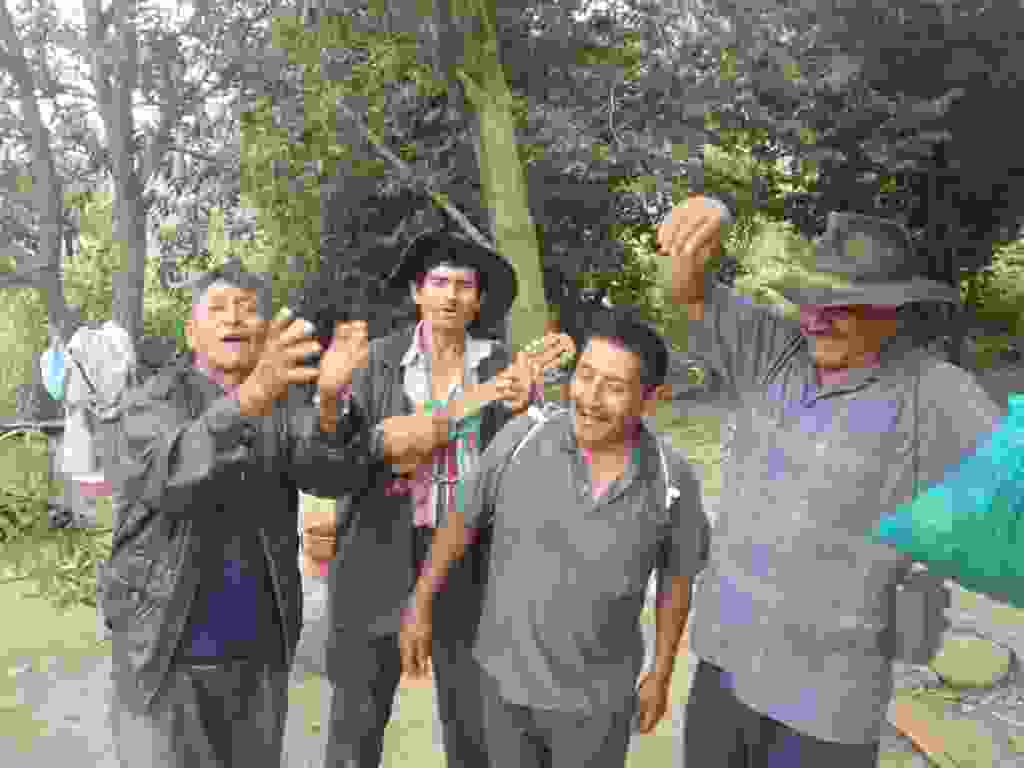
\includegraphics[width=\mywidth]{../wp-content/uploads/2015/04/wpid-wp-1429715261110-1024x768.jpg} \end{center}

 

 Puis j'arrive à Aiquile, la capitale du Charango la mini guitare sur la photo précédente. 

 

\begin{center} 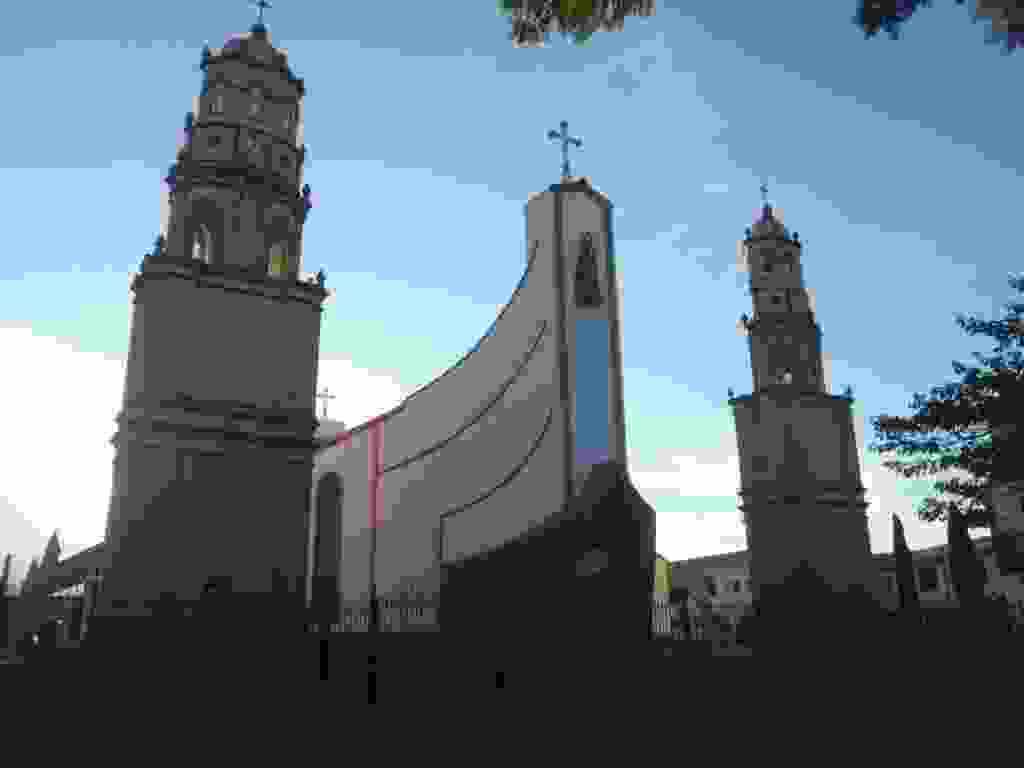
\includegraphics[width=\mywidth]{../wp-content/uploads/2015/04/wpid-wp-1429715491596-1024x768.jpg} \end{center}

 

 Je rencontre un nouveau type de route en pierre : pas très agréable ça secoue beaucoup. 

 

\begin{center} 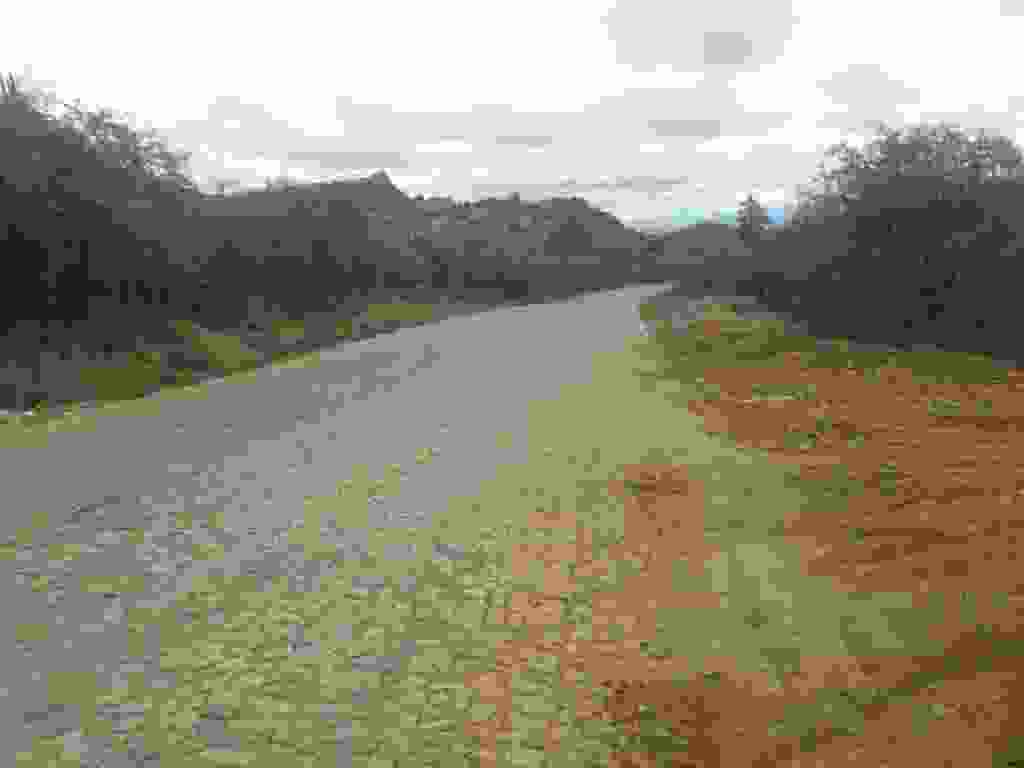
\includegraphics[width=\mywidth]{../wp-content/uploads/2015/04/wpid-wp-1429716153838-1024x768.jpg} \end{center}

 

 Le bord est plus roulant mais cette route est bordée d'arbustes avec des épines vraiment grandes. Au bout de 10km c'est la première crevaison du voyage. Je répare et en remontant c'est l'attache de la roue arrière qui casse. 

 Pas le choix je dois faire du stop, un camion s'arrête assez rapidement et par chance il va vers Cochabamba. C'est parti pour 200km à l'arrière du camion ! 

 

\begin{center} 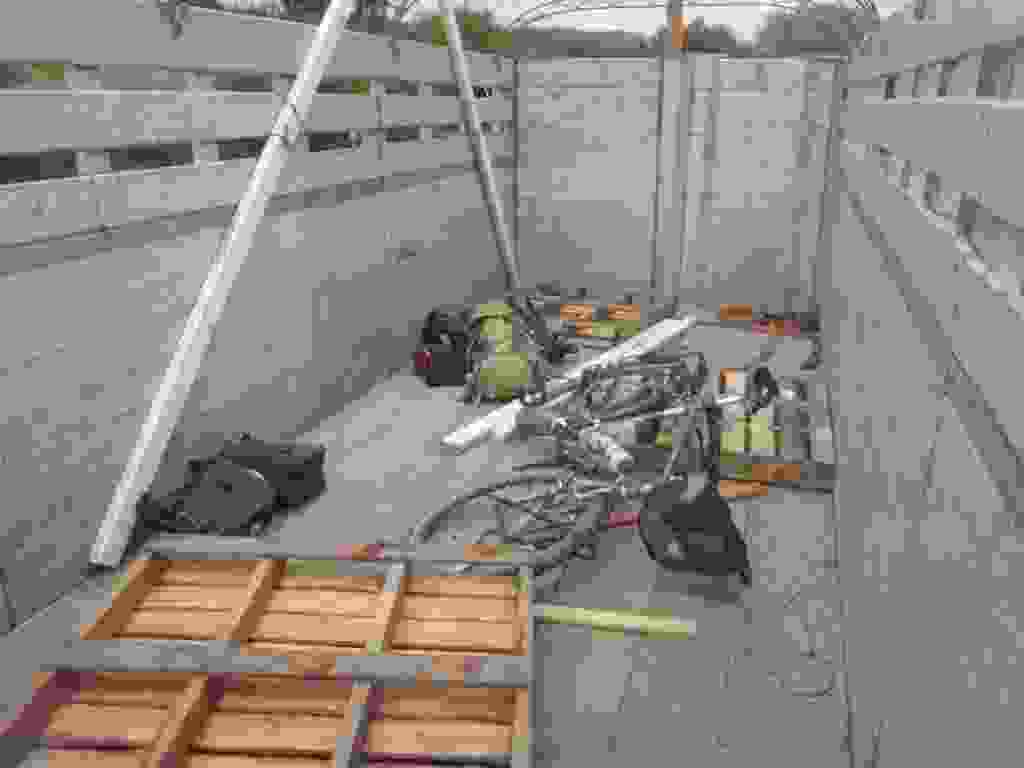
\includegraphics[width=\mywidth]{../wp-content/uploads/2015/04/wpid-wp-1429716662010-1024x768.jpg} \end{center}

 

 Je rate une belle portion de route à flan de montagne mais cela m´évite aussi de longues montées sur une surface difficile. 

 

\begin{center} 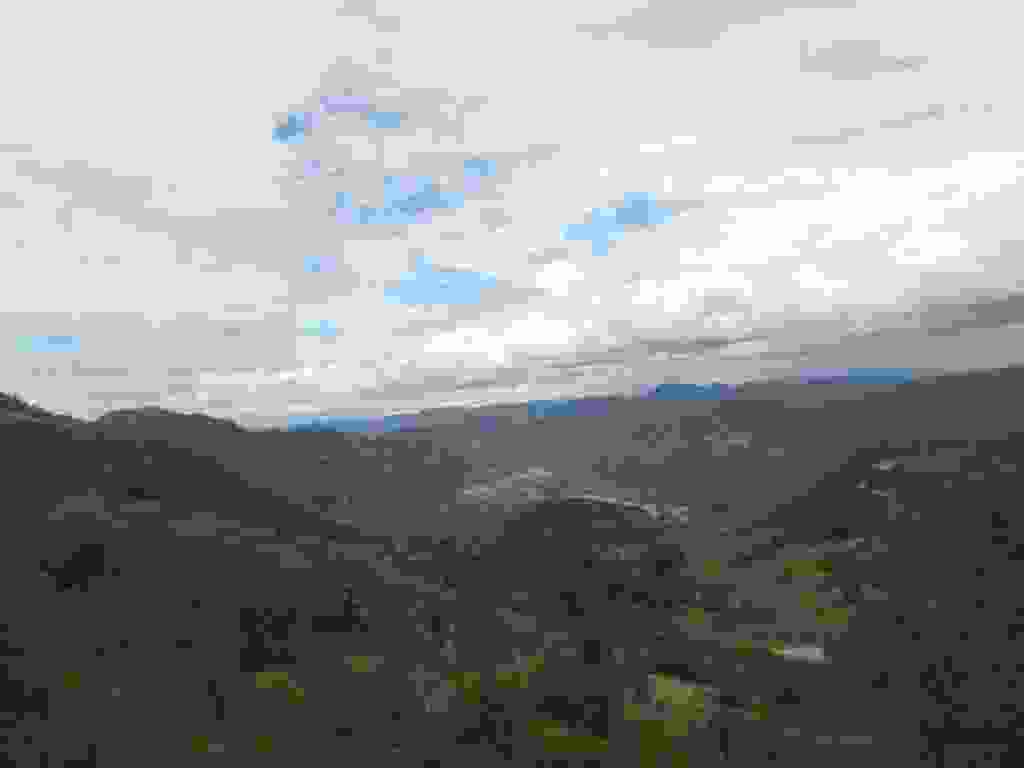
\includegraphics[width=\mywidth]{../wp-content/uploads/2015/04/wpid-wp-1429717092474-1024x768.jpg} \end{center}

 

 

\begin{center} 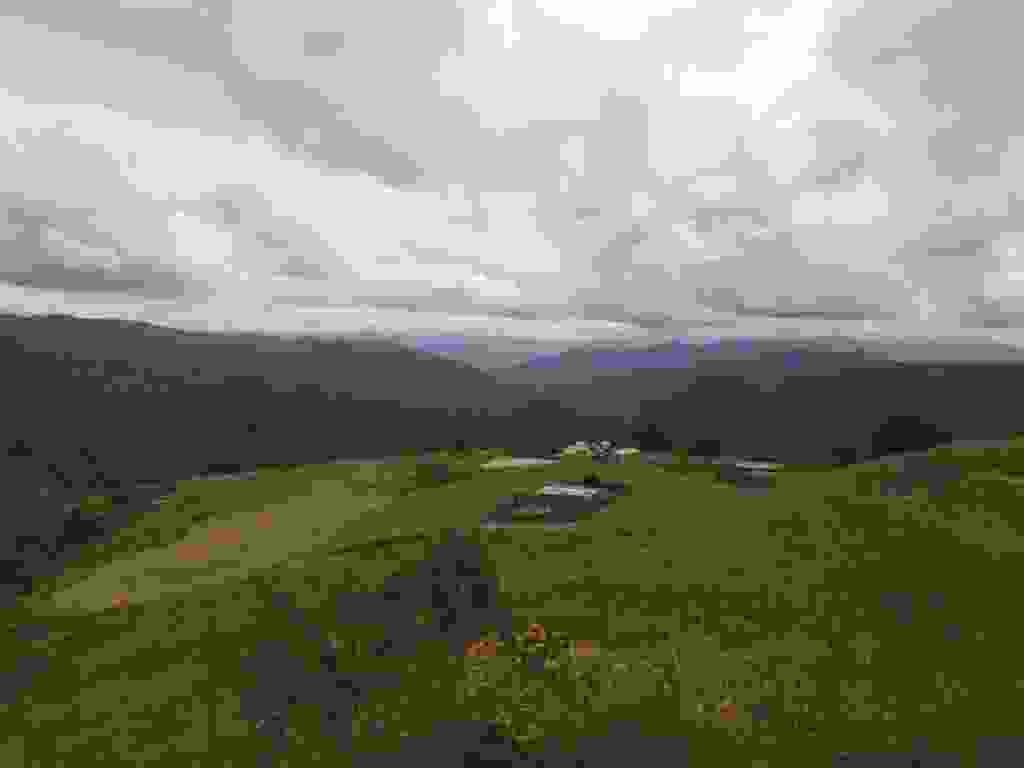
\includegraphics[width=\mywidth]{../wp-content/uploads/2015/04/wpid-wp-1429717103661-1024x768.jpg} \end{center}

 

 Du coup j'arrive plus vite que prévu à Cochabamba où je suis hébergé par Hache, américain de 75 ans qui a voyagé en vélo de nombreuses années. 

 

\begin{center} 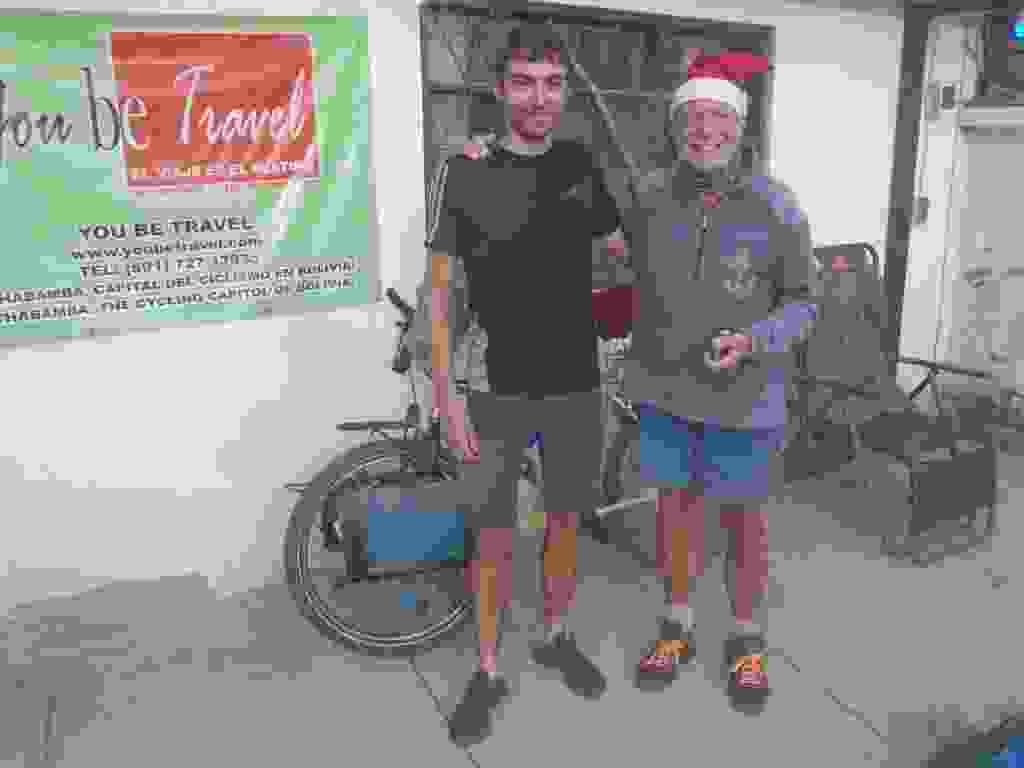
\includegraphics[width=\mywidth]{../wp-content/uploads/2015/04/wpid-wp-1430169754284-1024x768.jpg} \end{center}

 

 Je rencontre aussi Johnny, cycliste argentin qui vit là. 

 

\begin{center} 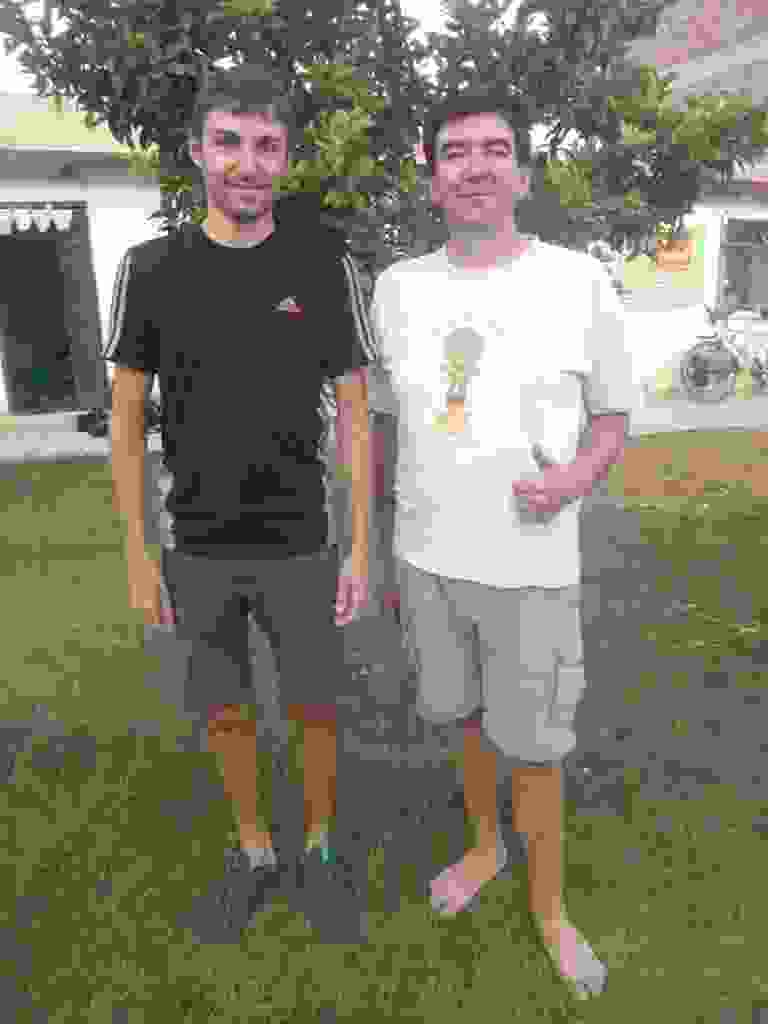
\includegraphics[width=\mywidth]{../wp-content/uploads/2015/04/wpid-wp-1430172032816-768x1024.jpg} \end{center}

 

 Ce très bon accueil me fait rester 1 semaine à Cochabamba qui est une ville peu touristique mais agréable. 

 

\begin{center} 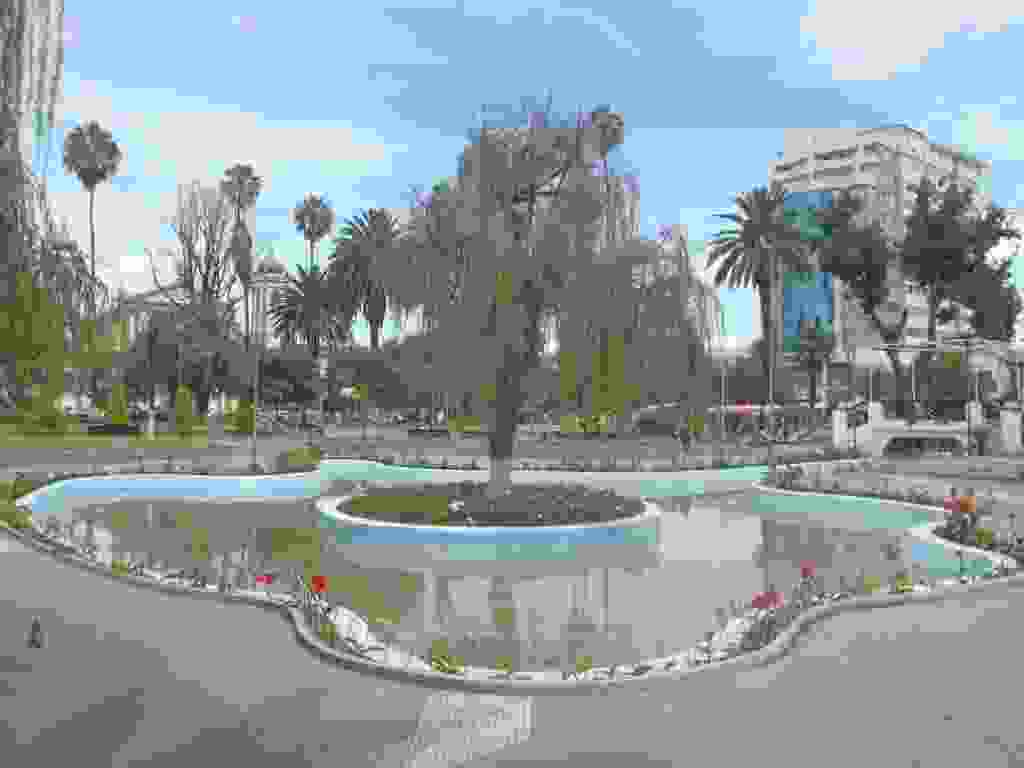
\includegraphics[width=\mywidth]{../wp-content/uploads/2015/04/wpid-wp-1430169894852-1024x768.jpg} \end{center}

 

 

\begin{center} 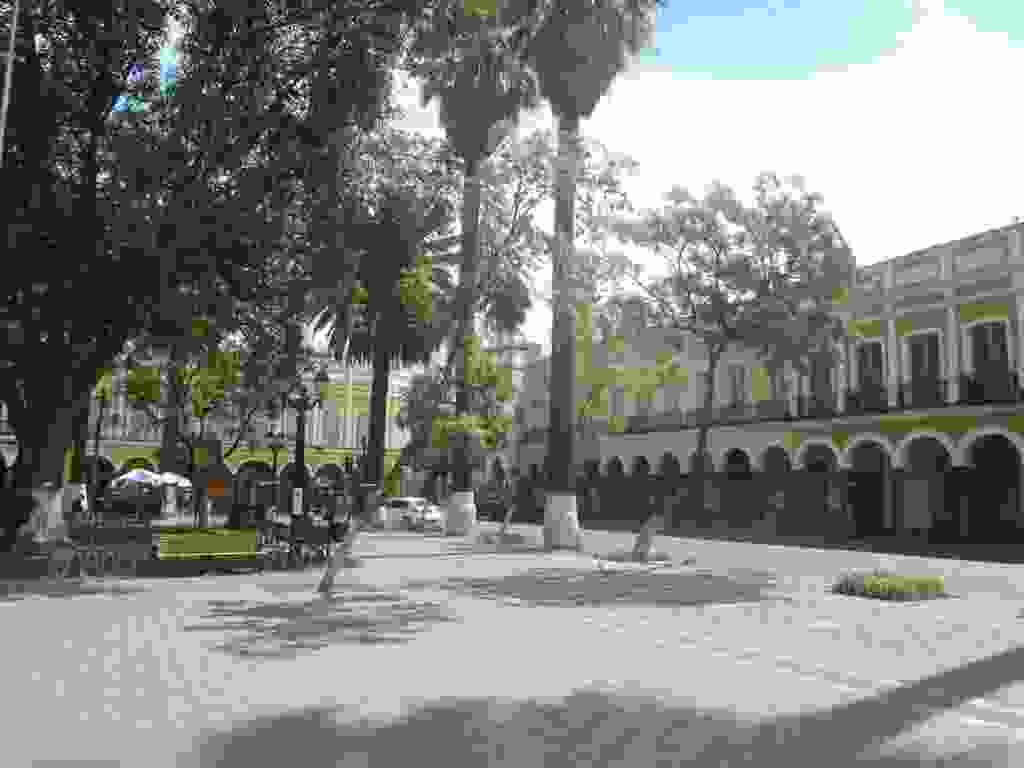
\includegraphics[width=\mywidth]{../wp-content/uploads/2015/04/wpid-wp-1430169968401-1024x768.jpg} \end{center}

 

 Montée au Christo de la Concordia. 

 

\begin{center} 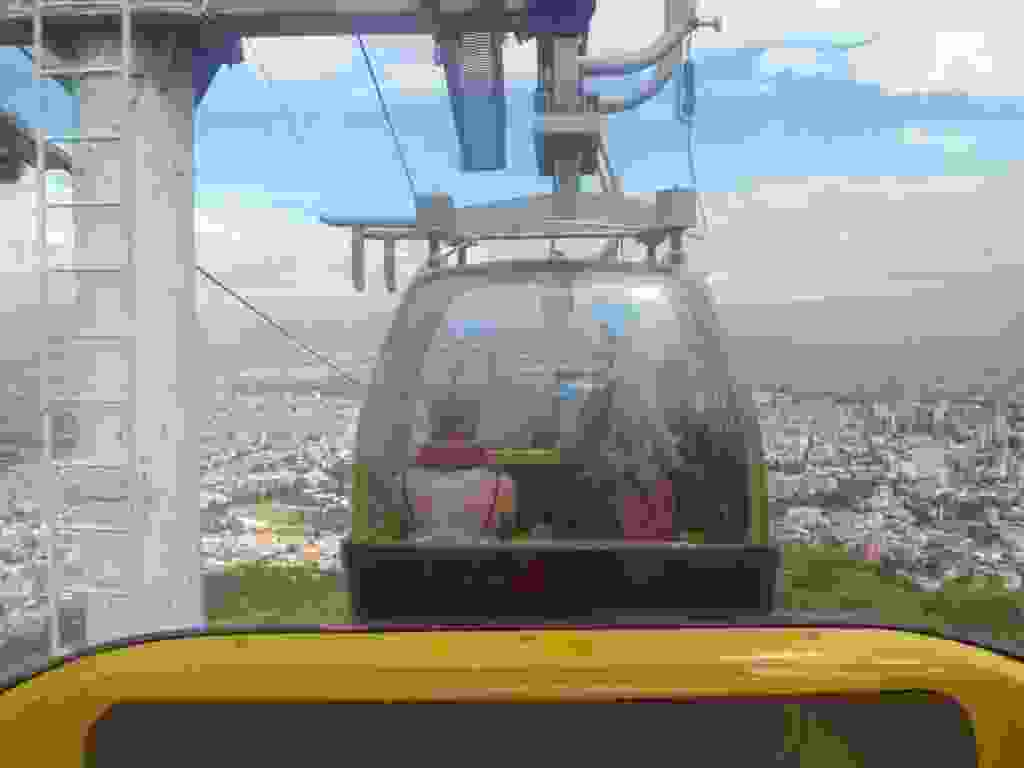
\includegraphics[width=\mywidth]{../wp-content/uploads/2015/04/wpid-wp-1430170103426-1024x768.jpg} \end{center}

 

 

\begin{center} 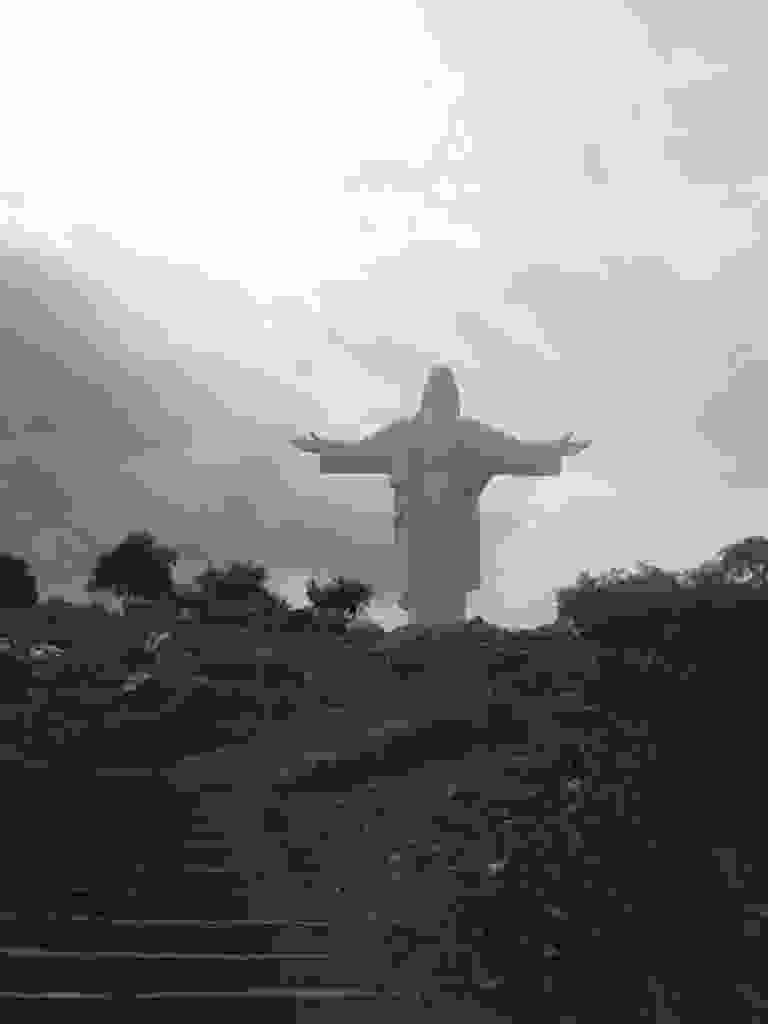
\includegraphics[width=\mywidth]{../wp-content/uploads/2015/04/P4213577-768x1024.jpg} \end{center}

 

 

\begin{center} 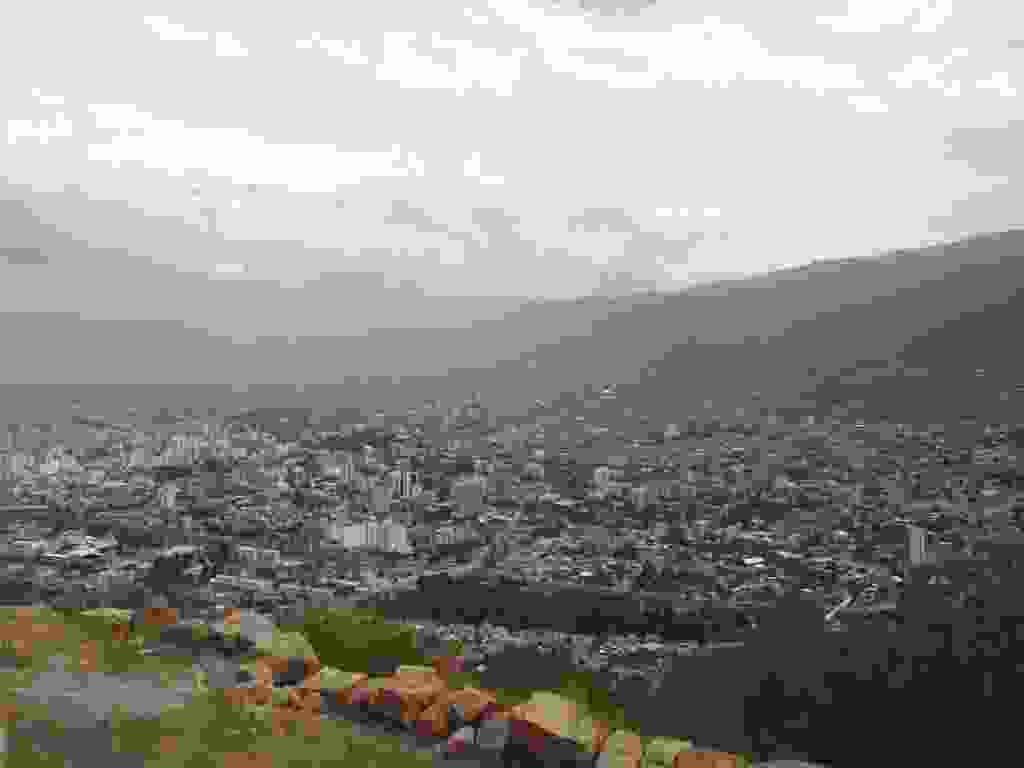
\includegraphics[width=\mywidth]{../wp-content/uploads/2015/04/P42135781-1024x768.jpg} \end{center}

 

 Le marché de la Cancha, immense. 

 

\begin{center} 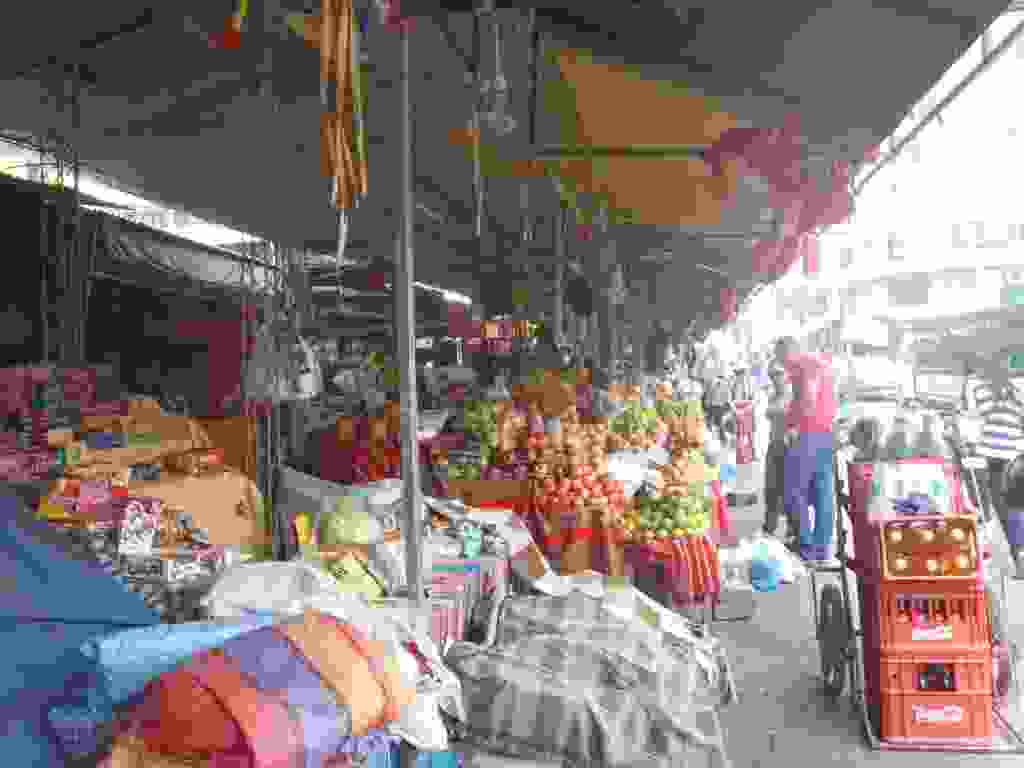
\includegraphics[width=\mywidth]{../wp-content/uploads/2015/04/P4213590-1024x768.jpg} \end{center}

 

 

\begin{center} 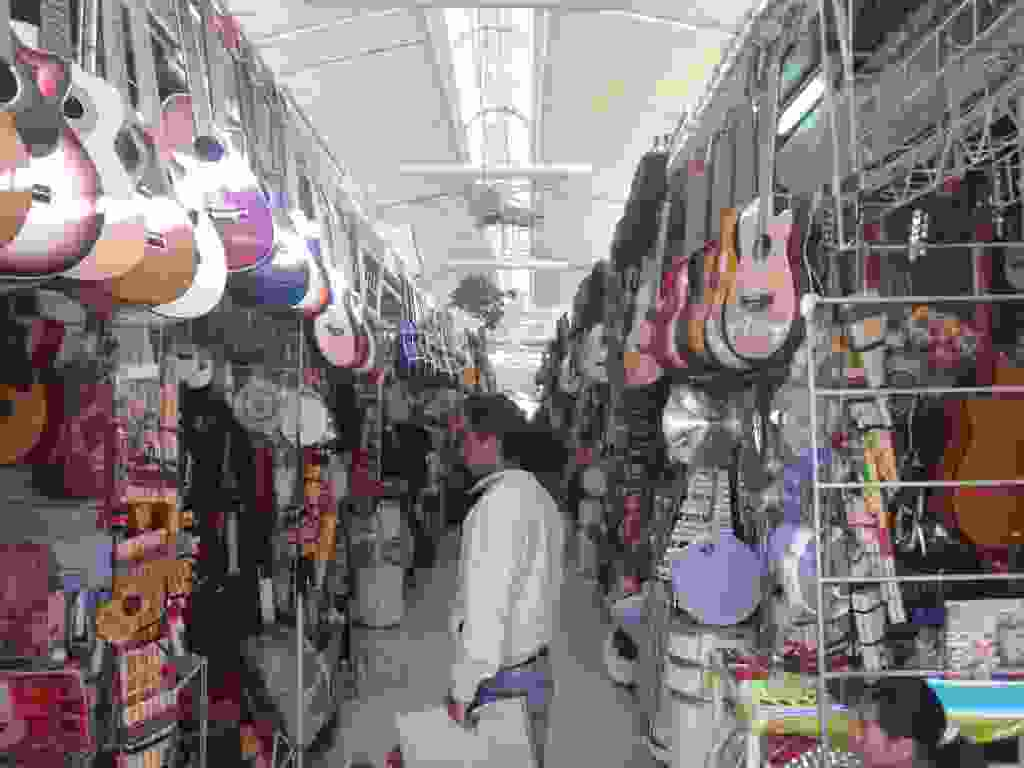
\includegraphics[width=\mywidth]{../wp-content/uploads/2015/04/P4213591-1024x768.jpg} \end{center}

 

 Le Palacio Portales construit par un bolivien ayant fait fortune dans le commerce de l'étain. 

 

\begin{center} 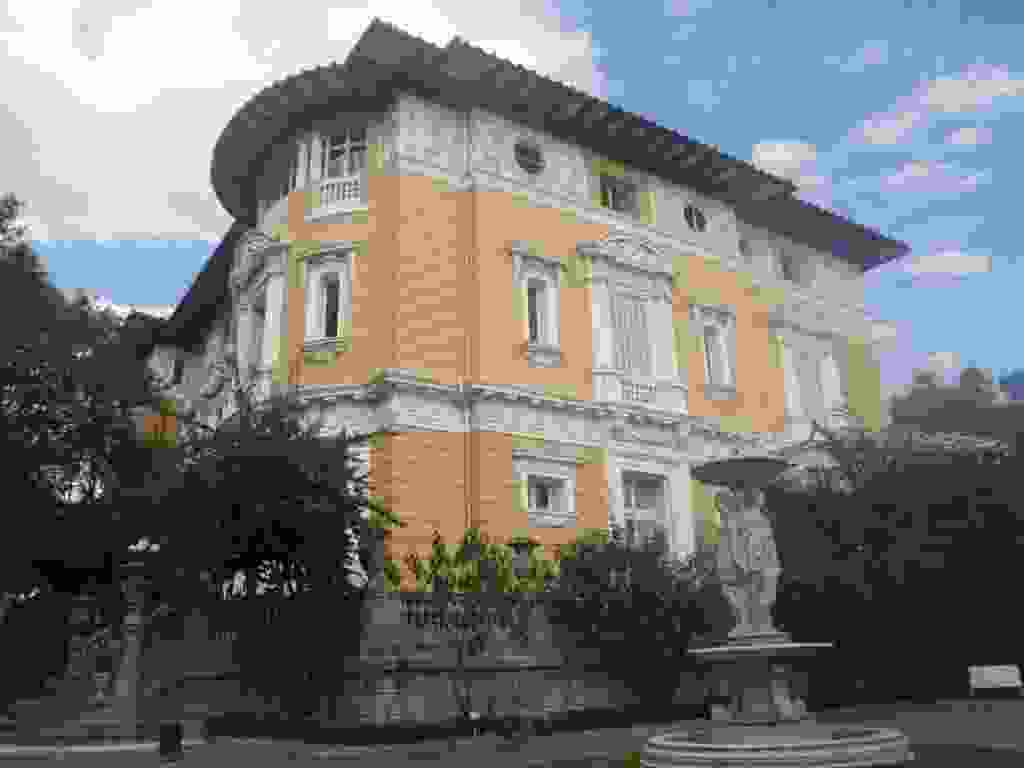
\includegraphics[width=\mywidth]{../wp-content/uploads/2015/04/P4213594-1024x768.jpg} \end{center}

 

 Pendant 2 jours je suis parti visiter le parc de Torotoro à 140km de Cochabamba. 

 

\begin{center} 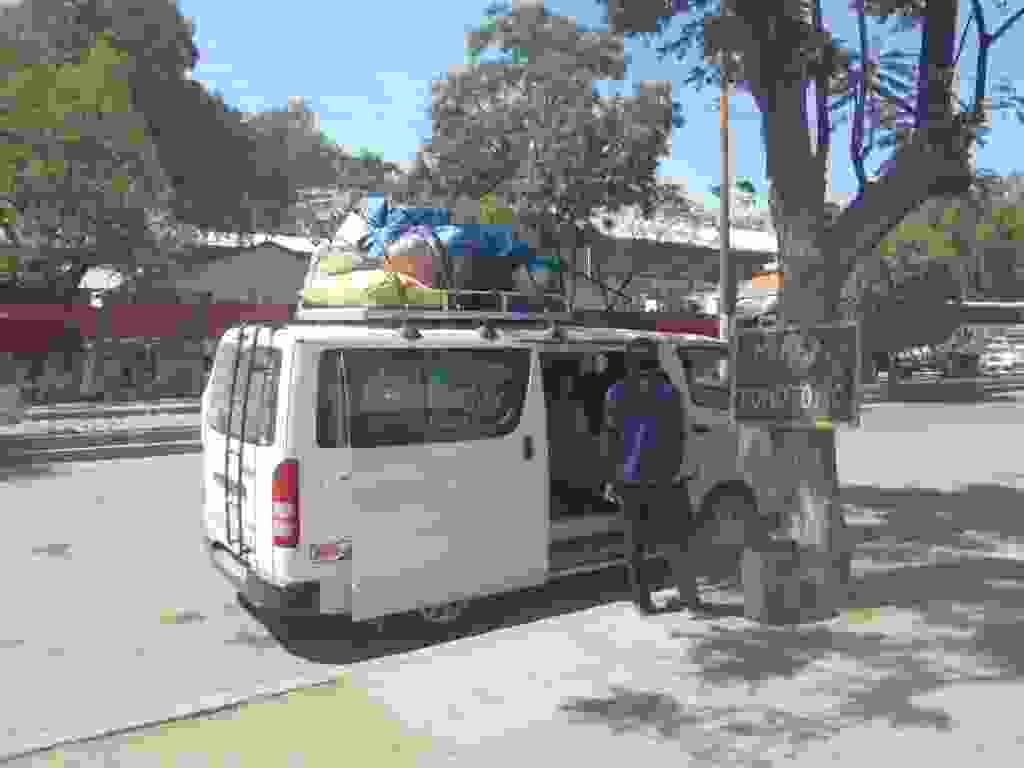
\includegraphics[width=\mywidth]{../wp-content/uploads/2015/04/P4243604-1024x768.jpg} \end{center}

 

 

\begin{center} 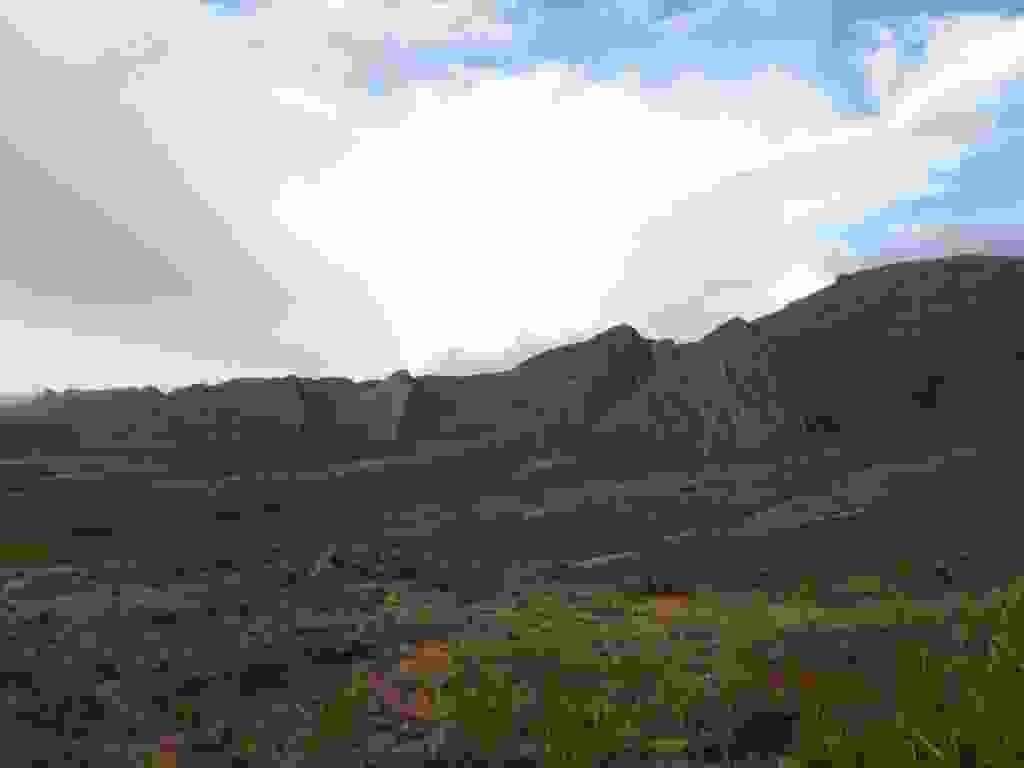
\includegraphics[width=\mywidth]{../wp-content/uploads/2015/04/P4253606-1024x768.jpg} \end{center}

 

 Le site de Itas : des grottes ayant été habitées pendant la préhistoire. 

 

\begin{center} 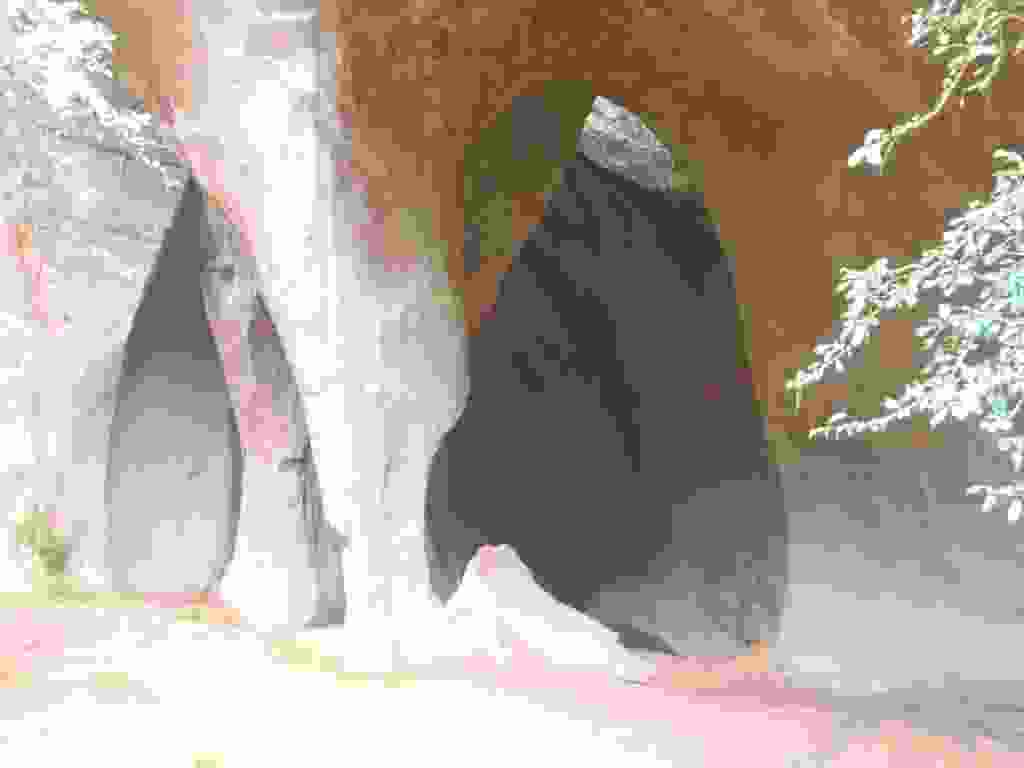
\includegraphics[width=\mywidth]{../wp-content/uploads/2015/04/P4253613-1024x768.jpg} \end{center}

 

 

\begin{center} 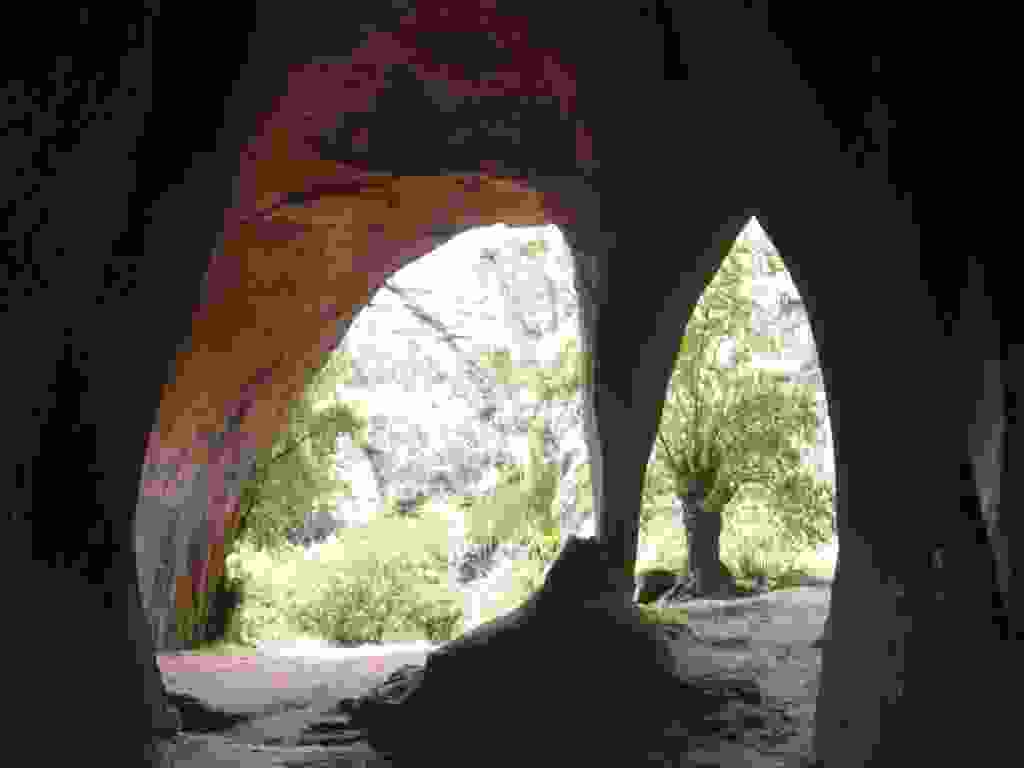
\includegraphics[width=\mywidth]{../wp-content/uploads/2015/04/P4253614-1024x768.jpg} \end{center}

 

 

\begin{center} 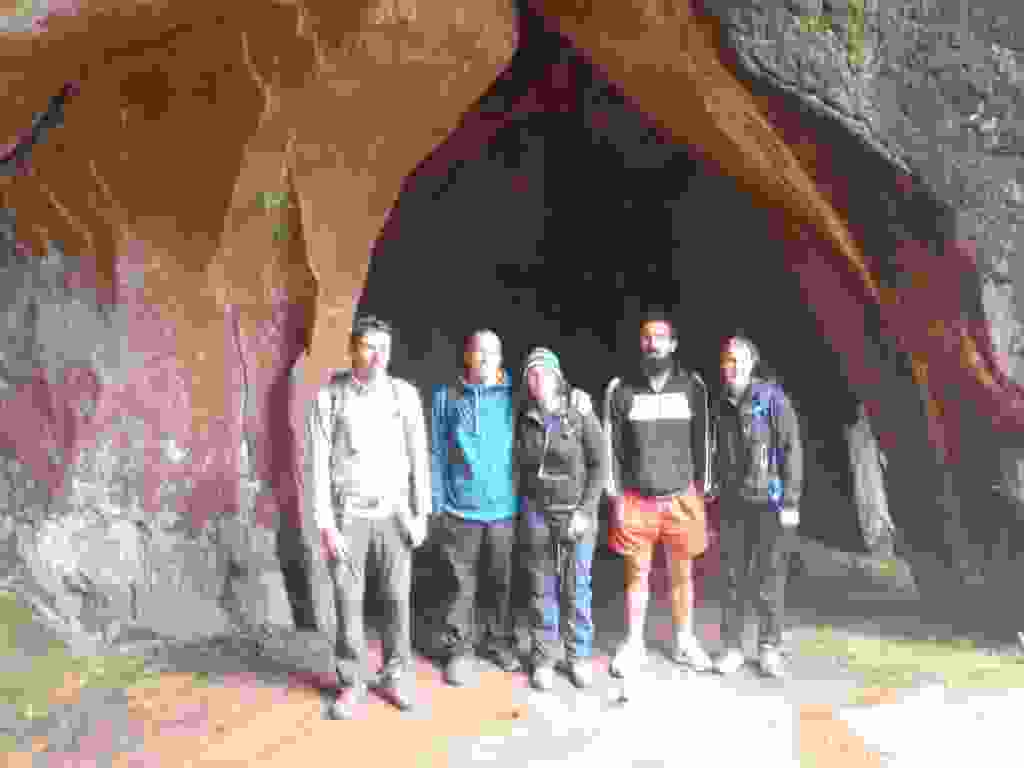
\includegraphics[width=\mywidth]{../wp-content/uploads/2015/04/P4253612-1024x768.jpg} \end{center}

 

 La grotte de Umajalanta : visite sportive avec des passages à plat ventre et escalades avec cordes. 

 

\begin{center} 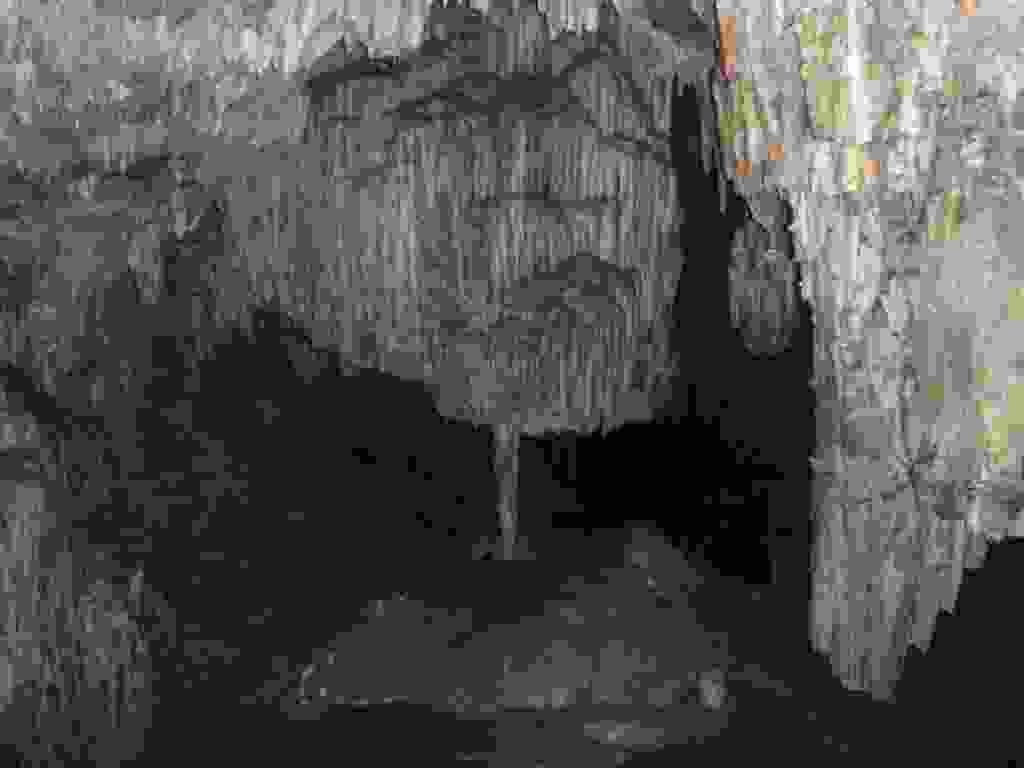
\includegraphics[width=\mywidth]{../wp-content/uploads/2015/04/P4253634-1024x768.jpg} \end{center}

 

 Ici pas de problème pour toucher les stalactites ou même s'y accrocher pour monter, de toute façon elles sont déjà toutes cassées. 

 

\begin{center} 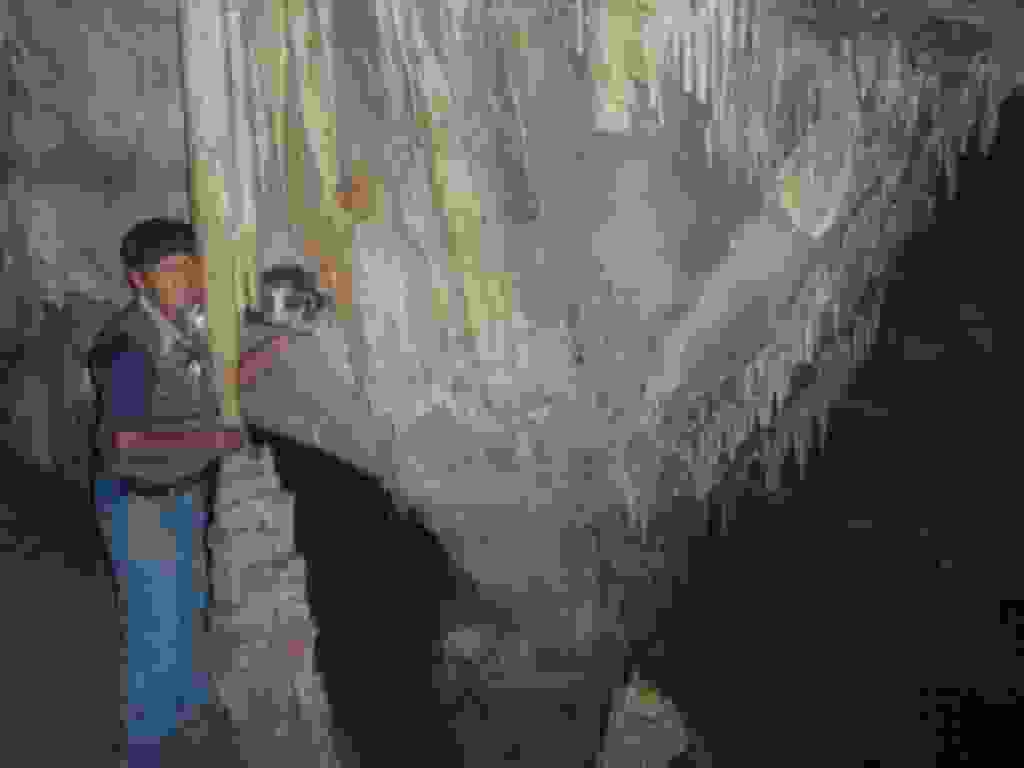
\includegraphics[width=\mywidth]{../wp-content/uploads/2015/04/P4253639-1024x768.jpg} \end{center}

 

 

\begin{center} 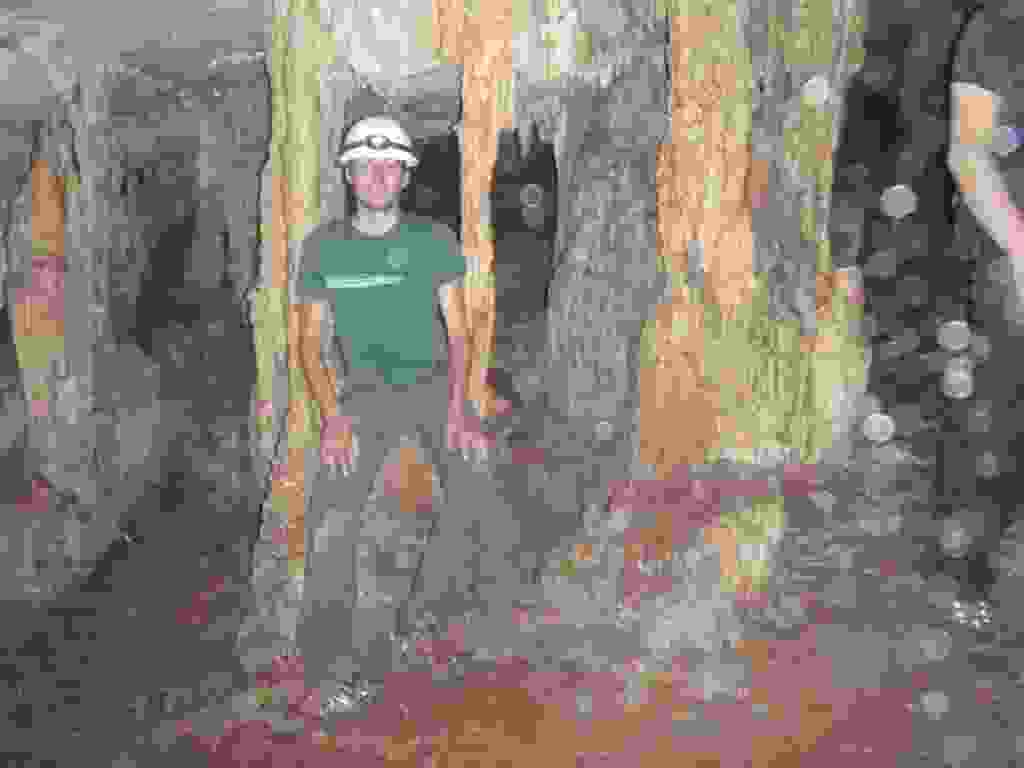
\includegraphics[width=\mywidth]{../wp-content/uploads/2015/04/P4253642-1024x768.jpg} \end{center}

 

 Randonnée au canyon de Vergel. 

 

\begin{center} 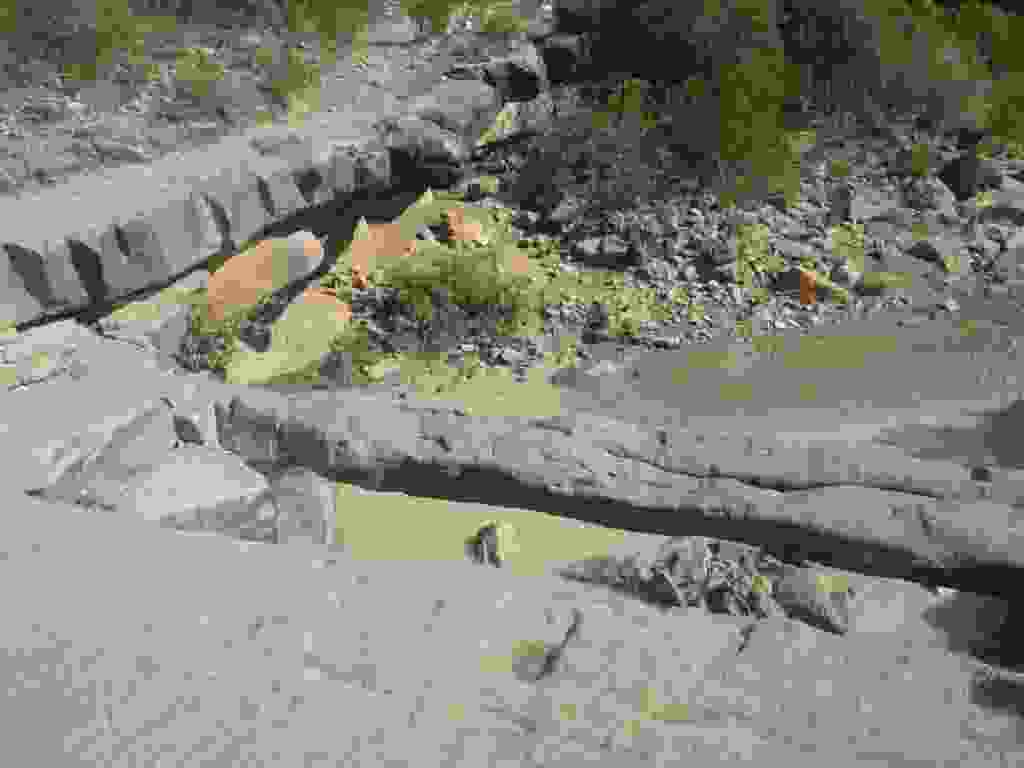
\includegraphics[width=\mywidth]{../wp-content/uploads/2015/04/P4263649-1024x768.jpg} \end{center}

 

 

\begin{center} 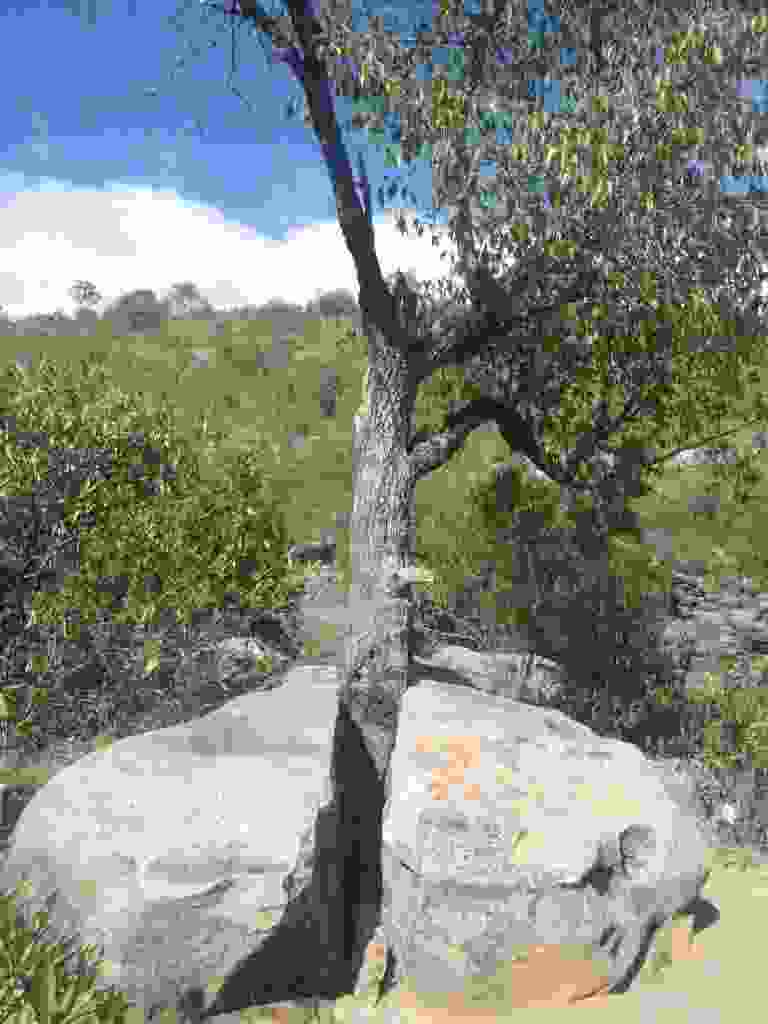
\includegraphics[width=\mywidth]{../wp-content/uploads/2015/04/P4263651-768x1024.jpg} \end{center}

 

 

\begin{center} 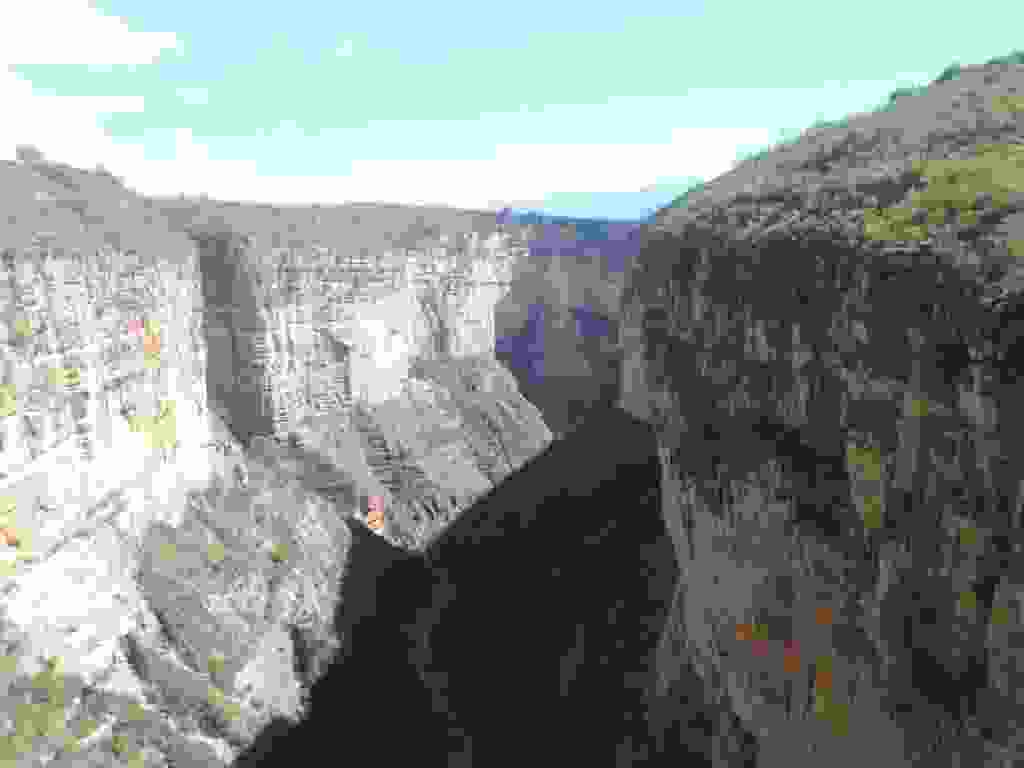
\includegraphics[width=\mywidth]{../wp-content/uploads/2015/04/P4263653-1024x768.jpg} \end{center}

 

 La descente au fond du canyon finit sur une belle cascade. 

 

\begin{center} 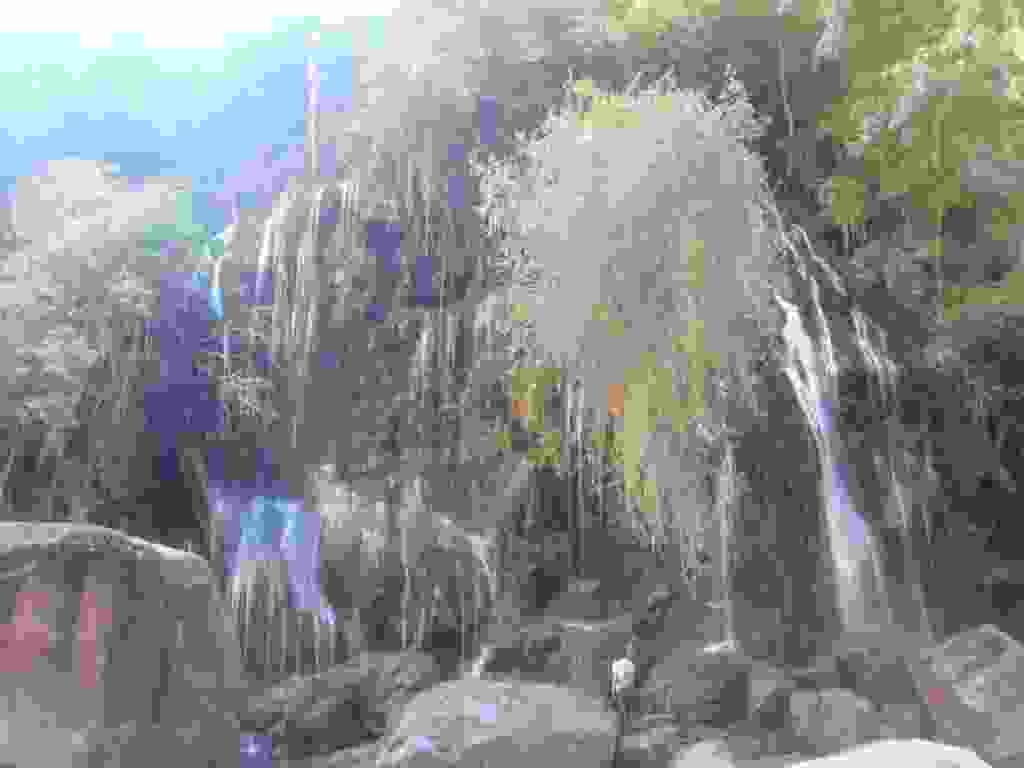
\includegraphics[width=\mywidth]{../wp-content/uploads/2015/04/P4263662-1024x768.jpg} \end{center}

 

 Le long du chemin, de nombreuses traces de dinosaures. 

 

\begin{center} 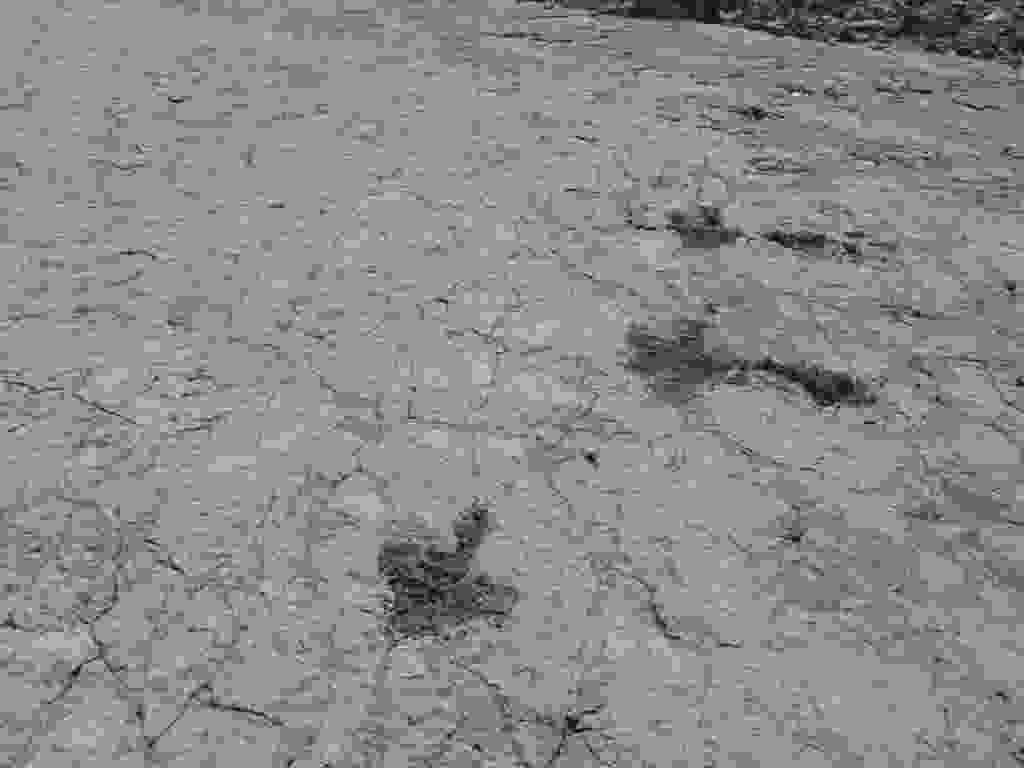
\includegraphics[width=\mywidth]{../wp-content/uploads/2015/04/P4253633-1024x768.jpg} \end{center}

 

 

\begin{center} 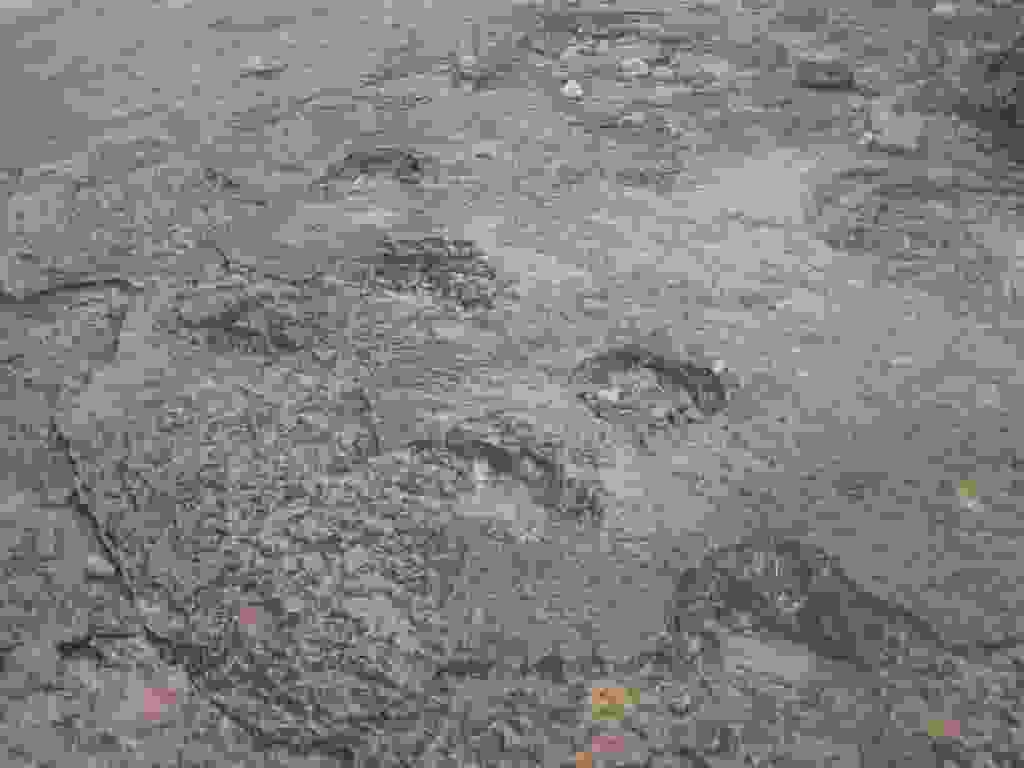
\includegraphics[width=\mywidth]{../wp-content/uploads/2015/04/P4263647-1024x768.jpg} \end{center}




 
 
